\chapter{Multi-Cloud-Anwendungs-Broker}

% Vorteile
% Neue Märkte in anderen Regionen der Welt
% Schnelles Ausrollen neuer Apps
% DevOps geeignet
% Risikoreduzierung
% Reduzierung von (gleichzeitig) Investitionsausgaben und Betriebskosten
% Bestehende Cloud-Deployments mit verwalten-

Um eine Anwendung automatisiert auf verschiedene Clouds zu verteilen ist ein Broker-Mechanismus nötig. Dieser sollte nach verschiedenen, festzulegenden Kriterien vorgehen. Konkret erfüllt ein Broker in der Regel folgende Aufgaben:

\begin{enumerate}
	\item Bereitstellen der Ressourcen für eine Applikation; starten einer virtuellen Maschine oder Reservierung von Speicherplatz
	\item Starten der Anwendung auf den vorher reservierten Ressourcen
	\item Verteilen eingehender Anfragen auf gestartete Anwendungs-Instanzen
	\item Management der Ressourcen
\end{enumerate}

\noindent
Zusätzlich sollte der Multi-Cloud-Broker Policys und SLAs auswerten und umsetzen können. Denkbar ist das automatische Re-provisionieren anhand von 

\begin{enumerate}
	\item Lastspitzen oder Ausfällen von Hardware und Netzwerkressourcen 
	%	(Monitoring)
	\item Geänderten Umfeldparametern wie der Gesetzgebung, Preisen oder AGBs
	\item Nutzeränderungen
	\item Vorherigen Broker-Aktionen
\end{enumerate}

\noindent
In einer Community Cloud könnten Cloud-Provider selbst einen Mechanismus zum Brokering oder zumindest offene APIs bereitstellen. Der Broker wäre also Teil der Cloud. Möglich sind entweder ein zentraler Broker, der direkt auf Cloud-Interna zugreift, oder aber ein Peer-to-Peer-Verbund.\todo{Grafik Architekturübersicht}

Für Multi-Clouds kommen diese Lösungen nicht infrage: Sie bestehen aus mehreren unabhängigen, meist privaten, Cloud-Providern. Aufgrund gegenläufiger Geschäftsinteressen sind diese nicht an einer Föderation mit anderen Anbietern interessiert. Sie werden also weder Interna ihrer Cloud-Plattform anpassen, noch einheitliche APIs bereitstellen.

Stattdessen muss der Broker in einer Multi-Cloud-Umgebung extern bereitgestellt werden. In diesem Fall kann er entweder als eigenständiger Service in Form einer \emph{Cloud Management Platform} angelegt sein, oder von der verteilten Anwendung selbst implementiert werden. Selbst entwickelte CMPs oder integrierte Broker setzen oft auf Multi-Cloud-Bibliotheken wie \emph{Apache libcloud}. \autoref{sec:bibliotheken} bietet hierzu eine Übersicht aktueller Open Source-Projekte. 

Folgende weitere Aspekte sollen bei der Betrachtung der CMPs berücksichtigt werden:

\begin{description}
	
	\item[Zielgruppe] 	\emph{Entwickler und Administratoren}: Im Rahmen von DevOps stellen sie verschiedene Ausführungsumgebungen für Entwicklung, Test und Produktion bereit. Dabei nutzen sie die Self-Service-Funktionen der CMPs.
	
						\emph{Management}: Die Auslastungs- und Kostenübersicht ermöglicht weitere Planung. SLAs und Policys werden überwacht und durchgesetzt.
	
	\item[Anwendungen] Grundsätzlich alle interaktiven Anwendungen und Dienste, sowie Stapelverarbeitungs-Jobs. Diese können verteilt sein, die CMP muss in diesem Fall z.\,B. die Nähe des Datenspeichers zur Rechen-Einheiten beachten.
	
	Ausgenommen spezielle Big Data Analytics und Forschungsszenarien, die unter Umständen besondere Features, Rechte und Architekturen benötigen.
	
	\item[Funktionsumfang] Über die grundlegende Provisionierung hinaus sollte die CMP auch bei weiteren Orchestrationsaufgaben unterstützen: Konfiguration, Monitoring und Skalieren.
	
	Die Unterstützung aktueller Container-Technologien und Cloud-Native-Architekturen ist wünschenswert. Keine Rolle spielt \emph{Bare Metal}: Eine installierte Virtualisierungsschicht oder Container-Laufzeitumgebung wird vorausgesetzt. 
	
	Die Auswertung der SLAs und Policys ist auf die verteilten Anwendungen selbst beschränkt. Darüber liegende (CMP-Nutzer) oder tiefergehende Schichten (Service-Nutzer und -Daten) werden extern verwaltet.
		
\end{description}


\noindent
Der folgende Abschnitt gibt eine Übersicht kommerzieller Cloud Management Plattformen sowie bisheriger Forschung zu Inter- und Multi-Cloud-Brokern mit besonderem Blick auf SLAs und Policys. Die vorgestellten Lösungen unterschieden sich in Architektur, Flexibilität und Funktionsumfang. Die vier Broker-Basiseigenschaften werden nicht von allen Arbeiten in vollem Umfang erfüllt.

Weiterhin zeigen wir einheitliche Ansätze zu maschinenlesbaren Policy- und SLA-Definitionen. Anschließend entwickeln wir ein Service-Schema für den Multi-Cloud-Einsatz. Es folgen der Vorschlag für ein Broker-Design und passende Matching-Algorithmen.

\section{Die Limitierungen Kommerzieller CMPs}

Kommerzielle Anbieter wie RightScale betonen den Self-Service-Charakter ihrer Cloud-Management-Lösungen: 
Im Vergleich zu virtuellen Maschinen
- Keine lange Wartezeit auf die Bereitstellung durch die IT
- Keine manuellen Konfigurationsarbeiten

Im Vergleich zur Cloud allgemein:
- Überblick über Preise
- Überblick über technische Angebote

Im Vergleich zu beiden:
- Durchsetzen von Policys
- Abbau der \emph{Schatten-IT}
- Kosteneinsparung durch bedarfsgerechte Ressourcenplanung



CMP sollte unabhängig entwickelt und betrieben werden. Cloud-Provider-eigene Lösungen nicht betrachtet. Und auf offene Standards setzen. Ansonsten ein neuer Single Point of Failure.

\todo{(Zusatz) Tabelle}

Bereitstellungsmodelle? Welche CMP ist nur als SaaS verfügbar?

Wie gut sind Features umgesetzt? Automatisierung oder nur schöne Dashboards?


\begin{description}
	
	\item[Red Hat CloudForms\footnotemark]\footnotetext{\url{https://www.redhat.com/en/technologies/management/cloudforms/}}
	Kommerzielle Cloud Management Platform, Grundlage ist das Open Source-Projekt  ManageIQ\footnotemark\footnotetext{\url{https://manageiq.org/}}, das alle wichtigen IaaS-Provider unterstützt (AWS, Azure, GCP, OpenStack).	
	
	Besonderheit: ein umfangreiches -- optional grafisches -- Policy-Management. Eigene Regeln folgen dem Schema \emph{Bedingung/Ereignis-Aktion}.
	
	Alle Schnittstellen der CMP sind proprietär. Die Orchestrierung liest jedoch vorhandene Vorlagen aus \emph{AWS CloudFormation} and \emph{OpenStack Heat}.
	%http://manageiq.org/docs/reference/latest/doc-Policies_and_Profiles_Guide/miq/
	
	\item[Rightscale CMP\footnotemark]\footnotetext{\url{https://www.rightscale.com/}}
	Proprietäres \emph{Software-as-a-Service}-Angebot, unterstützt alle wichtigen IaaS-Provider, zusätzlich Plattformdienste, Docker-Container und Hypervisoren, besonders \emph{VMware vSphere}.
	
	Infrastruktur und Dienste werden als Vorlagen in einem eigenen Katalog bereitgestellt. Dabei erlaubt Rightscale auch heterogene Anwendungen über IaaS-, CaaS- und PaaS-Grenzen hinweg.
	
	Ein Dashboard zeigt Empfehlungen zur Kostenoptimierung, allerdings ohne SLAs einzubeziehen.
	
	\item[Scalr] description

	%	Whitepaper! 
\end{description}

% https://www.embotics.com/solutions-cloud-governance
% Nur Azure und Amazon. Cloud Governance: Die richtigen Meta-Tags zu Instanzen hinzufügen. Kostenoptimierungsvorschläge, aber nur die Wahl zwischen zwei Providern.


Commercial (Rightscale) 

only trigger-action, no SLAs 



DivvyCloud (Commercial) 

Automation Bots to schedule downtime, terminate, or re-size instances and resources so you only pay for what you use 

https://divvycloud.com/product/botfactory/for-cost/ 

%
%Commercial Tools 
%
%https://www.cloudyn.com/ 
%
%close-source 
%
%only cost monitoring and optimization 
%
%Also, Rightscale, Cloudhealth, CloudCheckr 


Apache Scalr (complex, freemium) 

\section{Bisherige Forschungsarbeiten}

%policy-driven service placement optimization in federated clouds 


RESERVOIR (hard and soft requirements) 



OPTIMIS (Trust/Risk/Eco/Cost) 

canceled research project 

Dependable sociability = trust + risk + eco + cost 

introducing new multi-cloud HYBRID architectures with broker 

combination of federation and multi-cloud 

no geo-location 

non-disclosed algorithm 

no current external adapter available 

SP and IP, focus on IP benefit 





Contrail 

Federation 

Meta-data access (location, price..) 

although not usable in SLAs  :( 



Meryn 

SLA-driven PaaS system 

Optimize Cloud Provider costs 

Cloud Bursting 

Batch-application-centered (Hadoop) 

Single-use VMs 

Bidding 



InterCloud 

Pricing-aware 

Broker 

Federation 



Seaclouds EU project 

2013 

Cloud agnostic PaaS 

Discover/Planner/Deploy/Monitor/SLA-Services 

only monitors user-specific SLA 

Not used during planning/matchmaking 



Mist.io 

Open source 

Build on libcloud and cloudify 

Can monitor costs (commercial) 

No automatic scheduling 



An SLA-based Broker for Cloud Infrastructures 

Nicht nur Private Clouds sondern auch Personal Devices 

Modulare Architektur 

Fokus auf Föderation. Aber: Idee der forced integration of commercial cloud providers 

-> Mithilfe libcloud umsetzen 




Einige unterstützen über Adapter mehrere Bereitstellungsmodelle; je nachdem, ob dem Cloud-Provider die Mitgliedschaft in einer Föderation bewusst ist. Interne Adapter sprechen mit zusätzlichen, Cloud-internen Erweiterungen. Externe Adapter nutzen die öffentlichen APIs von Drittanbieter-Clouds.


Fazit: Die bisherigen Forschungsprojekte unterstützen keine Container-Technologien. Aus aktuellen \emph{DevOps}-Szenarien sind diese jedoch unverzichtbar.

Unterschiedliche Ausrichtung von Forschungsprojekten und Kommerziellen Anbietern Grozev: Forschungsprojekte fokussieren sich auf Föderationen. Dies entspricht auch dem vorherrschenden Cloud-Typ innerhalb der Projekte. SLAs werden ausschließlich von diesen ausgewertet und teilweise umgesetzt. Kommerzielle Projekte sind dagegen meist externe Broker, stellen Preisunterschiede und Kosten dar. Statt SLAs setzen sie nur einfachere Policys um.

Grozev: Universelle SLA-Spezifikation nötig

Code nur teilweise OpenSource, Matching nicht offengelegt. Nachvollziehbare Forschung sieht anders aus!

Proprietäre Schemata für Infrastruktur, Services und wenn verfügbar SLAs. 

APIs sind nicht einheitlich.

Kombination aus Pricing und Compliance bisher einmalig.






\section{Maschinenlesbare SLA- und Policy-Schemata}

Aufgreifen der Policy- und SLA-Anforderungen

Offen ist der Durchsetzungspunkt der Policys. Soll dies bereits in der CMP oder innerhalb von Plattformdiensten und Anwendungsprogrammen geschehen? Für Benutzer-Policys könnte beides der Fall sein: Die versendeten Anwendungsdaten enthalten Metainformationen zur erlaubten Verwendung. Schon die erste Kontaktstelle der Cloud, zum Beispiel ein Load-Balancer, wertet diese Informationen aus und entscheidet entsprechend für ein Routing, dass den Nutzeranforderungen entspricht. 

In der Anwendung selbst können diese Metainformationen auch genutzt werden, zum Beispiel zur gewünschten Verschlüsselung oder einer Frist zur automatischen Löschung. Ein besonders auf Performance fokussierter Ansatz ist [CPPL]. Bei System-Policys ist die Performance der Dekodierung jedoch nicht entscheidend: Sie findet nur bei Änderungen durch Administratoren statt, nicht bei jedem Datenpaket, das die Cloud erreicht.

Operational Level (Management, Computational)
Policy- und Event Definition Language
Anforderungen->Graph
% [2] T. Koch, C. Krell, and B. Krämer, "Policy definition language for automated management of distributed systems," In Proceedings of Second IEEE International Workshop on Systems Management, 1996, pp. 55-64.

CPPA (SCICLOPS) End User - Object privileges on 
Tables 
Indices 
Procedures 
SQL operations, e.g.,  
Select 
Insert 
Update 
Delete 
Create… 

System-Privilegien: Anwendungsverteilung, also Sicht eines Administrator
Admin - System privileges 
System and Application Setup 
User Management
Monitoring/Logging
Backup

Bisherige Standards

CSA, OPTIMIS

einfach lesen für Mensch und Maschine, Versionsverwaltung, Infrastruktur als Code, erweiterbar

\section{Einheitliche Infrastruktur- und Service-Definitionen}

Durch die Definition von SLAs und Policys steht nun fest, wo und wie ein Service bereitgestellt werden soll. Die konkrete technische Umsetzung ist bisher allerdings offen. Oberstes Ziel der CMP-Service-Definition ist Portabilität: Die gleiche Anwendung muss auf verschieden Hypervisoren, IaaS/CaaS- und Plattform-Angeboten ausgeführt werden. Nur so ergeben sich die Vorteile der Multi-Cloud-MP:

\begin{description}
	
	\item[Notfallplan] Bei Ausfall der gesamten Ausführungsplattform kann eine Migration zu einem anderen Anbieter erfolgen.
	
	\item[Abfangen von Lastspitzen] Zusätzliche Service-Instanzen auf externen Ressourcen bearbeiten bei Bedarf weitere Anfragen.
	
	\item[Lebenszyklus-Verwaltung] Typischerweise durchläuft eine neue Service-Version die Phasen Entwicklung, Test, Qualitätssicherung und Produktion. Hierfür existieren oft unterschiedliche Ausführungsumgebungen.
	
\end{description}

%Rightscale Video: https://www.rightscale.com/solutions/problems-we-solve/self-service-it

\noindent
Diese Vorteile ergeben sich jedoch nur, wenn sich die Anwendung auch für eine Cloud-Nutzung eignet. Je nach Entstehungsgeschichte können sich Software-Architektur und Migrations-Maßnahmen grundlegend unterscheiden:

\begin{description}
	
	\item[Klassisch] (Legacy-)Anwendung mit monolithischem Design
	
	$\Rightarrow$ Ausführungsumgebung portabel bereitstellen, z.\,B. als (Container-)Image
	
	\item[Web App] Mehrere skalierbare Komponenten
	
	$\Rightarrow$ Zusätzlich die Nutzbarkeit von PaaS-Komponenten prüfen
	
	\item[Cloud-Native] Abhängigkeiten zu proprietären Cloud-Services (interner Broker)
	
	$\Rightarrow$ Refactoring und Öffnung der Schnittstellen zur CMP
	
\end{description}

\noindent
Gerade bei klassischen, monolithischen Anwendungen ergeben sich Architektur-bedingt nicht alle Vorteile der Cloud-Nutzung; Eine erhöhte Portabilität ist gegeben --  Skalierbarkeit allerdings nicht. Die Entscheidung für Anpassung, Migration oder unverändertem Weiterbetrieb muss also je nach technischer Eignung und langfristiger Bedeutung für das Kerngeschäft abgewogen werden.

Vergleich Docker Compose usw.
Je nach Typ: Hypervisor/IaaS/CaaS/PaaS

Einige größere Verbreitung: Zum Beispiel AMI (Amazon Machine Images) und CloudFormation (Service-Definitionen)

Können sich jedoch jederzeit ändern. Nicht immer 100 prozent kompatibel.

Besonderheiten der zugrundeliegenden Provider-Infrastruktur. 

Eigenheiten der eigenen Plattform nicht nutzbar.

\todo{Schaubild Template-Level: Skripte/Variablen, Multi-Cloud Image/Container, IaaS/CaaS, PaaS}

Cloud Foundry PaaS (Theoretisch), aber nur PaaS, Migration von Monolithen unmöglich. Daher Kombination aus Hypervisor/IaaS/CaaS und PaaS nötig.
%https://blog.gruntwork.io/why-we-use-terraform-and-not-chef-puppet-ansible-saltstack-or-cloudformation-7989dad2865c 
Standard:
Multi-Cloud Images und Cloud-Init
Docker Container (Kubernetes, OpenShift)

Maybe packer: Build Automated Machine Images for both.

%Inspired by 
%
%Docker compose %
%Juju https://jujucharms.com/canonical-kubernetes/ %
%Terraform % SaltStack -> Just Infrastructure
% Chef Puppet Ansible -> Configuration (Shouldn't need those)
%Kubernetes https://kubernetes.io/docs/tutorials/stateless-application/guestbook/ But that is just for deployment of Docker Images on already existing Kubernetes Clusters. Not Multi-CLoud from Scratch! %
%http://docs.getcloudify.org/4.2.0/blueprints/spec-policy-types/ %
%https://en.wikipedia.org/wiki/OASIS_TOSCA (Cloudify/SeaClouds) 

Cloudify implementiert den TOSCA-Standard. Mithilfe (grafischer) Werkzeuge lassen sich Cloud-Infrastrukturen und Services modellieren. Plugins erweitern Cloudify um alle wichtigen Provider auf IaaS-Ebene (AWS, Azure, GCP, OpenStack) als auch CaaS (Docker, Kubernetes). Konfiguration wie das Start-Skript kann direkt übergeben, oder über ein Tool wie Puppet weitergeleitet. Optionale(?) AGents of Hosts. Built-in Policies and rudimentäres Monitoring über Plugins.

Komplex, aber vielversprechend. Hierauf aufbauen (eigenen YAML-ENtwurf erwähnen) und Brokering hinzufügen. Hier muss festgelegtw erden, welcher Service-Teil auf welchem Provider mit welchem Instanz-typen bereitgestellt werden soll. Dies soll automatisiert anhand von SLA/Policy und Preis entschieden werden. Unterstützt TOSCA deklarative Service-Definitionen?

Übernehmen?

Wie ist der STandard aufgebaut? Werden alle CLoud-EIgenheiten unterstützt?

%Read and Link Paper!

Portable Skripte und offene Schnittstellen (REST)
- Ersteinrichtung, Konfiguration und Start
- Änderung der Parameter im Betrieb
- 

Deklarativ: Laufendes Setup entspricht genau der Service-Definition
Agent-less: Weitere Anpassungshürden vermeiden

Wie kombinieren und Service-Komposition definieren?

Einige weitere technische Herausforderungen löst der Multi-Cloud-Broker: Management von SSL-Zertifikaten, statischen und virtuellen IPs, sowie Load Balancing. Andere Migrationshürden bleiben: Verfügbarkeit von Betriebssystemen, Frameworks und Bibliotheken, ebenso wie die Vereinbarkeit mit vorhandenen Lizenzen.



\section{Modularer Architektur-Vorschlag}

Komponenten des Brokers.


In der CMP: Polling oder Notification?

Was löst eine Aktion aus?
- Monitoring der Services
- Änderung der Umgebung
- User-Aktion
- Ergebnis einer anderen Policy

\begin{figure}
	\centering
	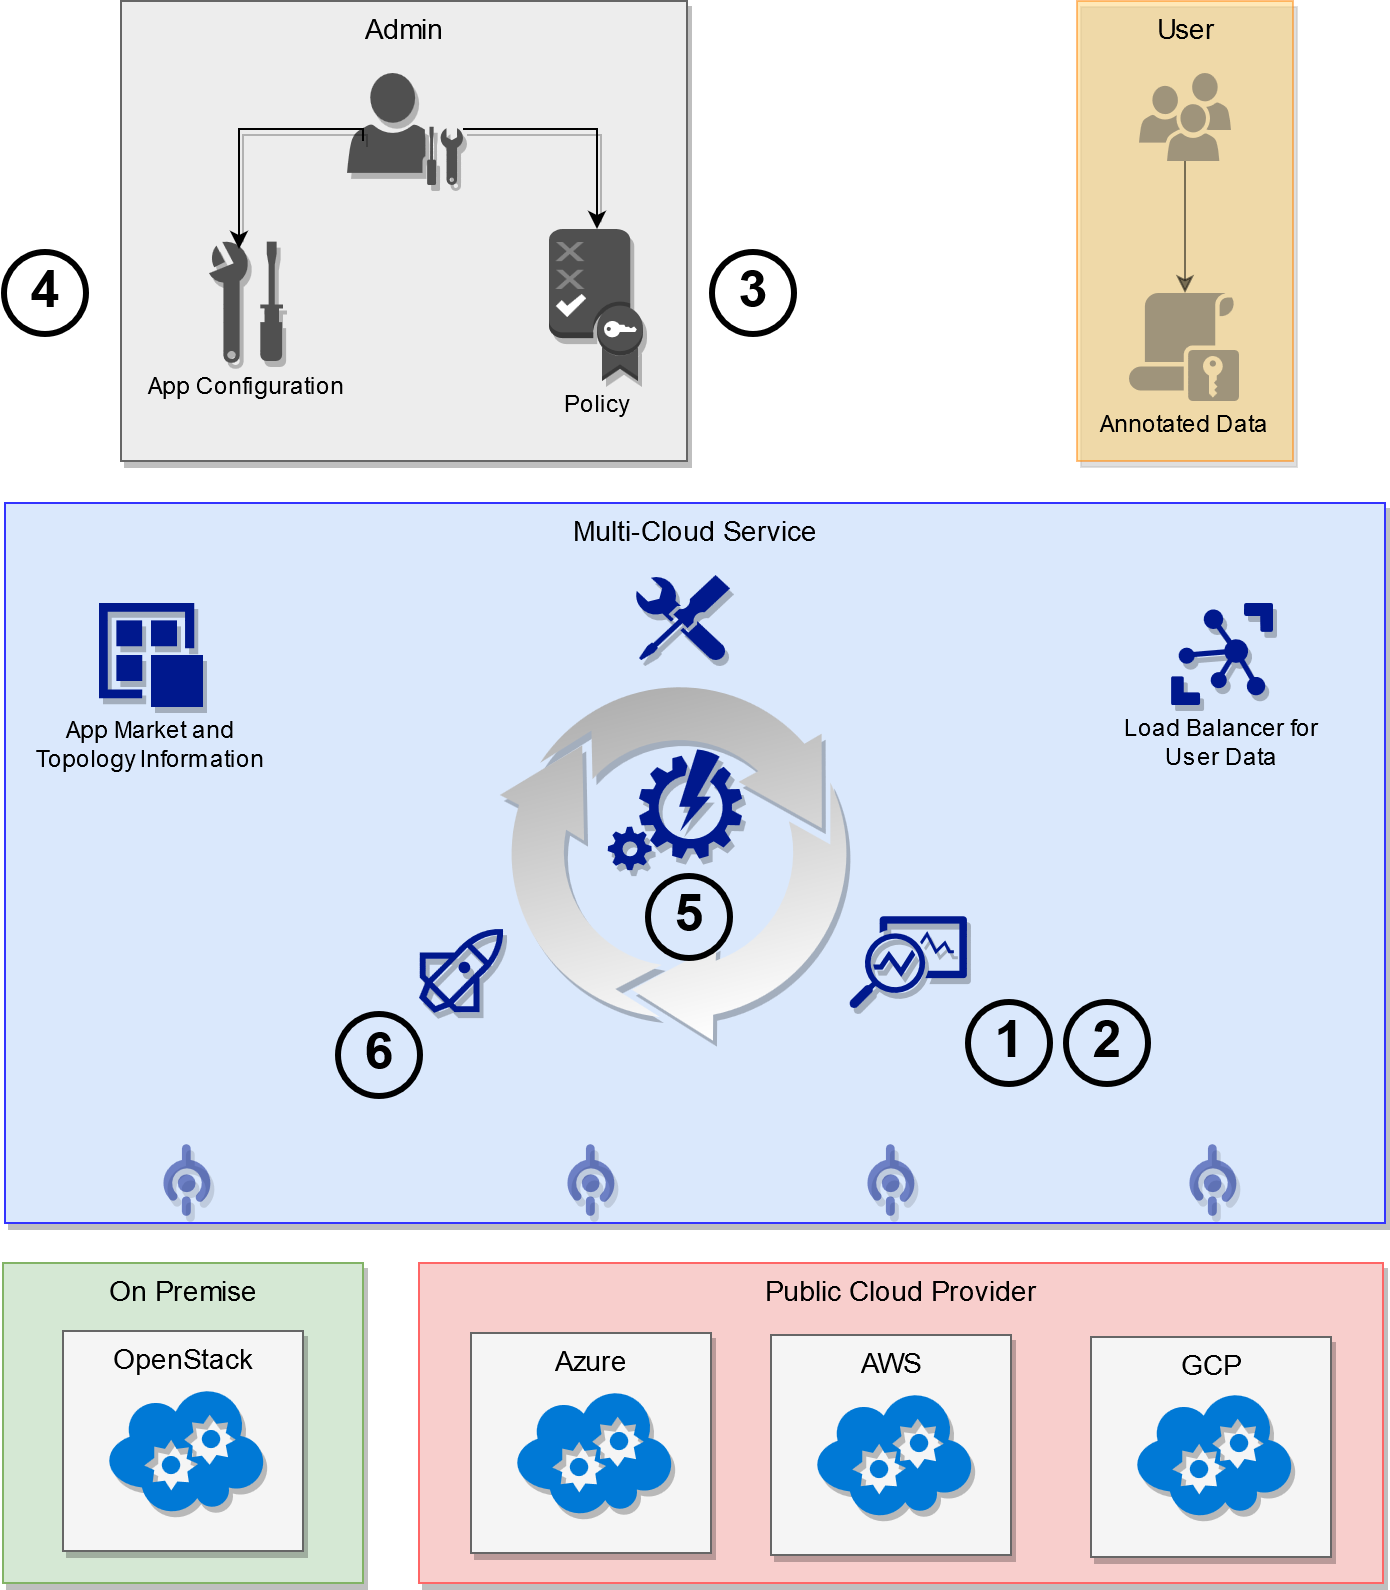
\includegraphics[width=0.9\linewidth]{images/cycle}
	\caption{}
	\label{fig:Chicken1}
\end{figure}

Zyklus\autoref{fig:Chicken1}:

%\begin{description}
%	\item[Nummerierte Aufzählung]~\par
\begin{enumerate}
	
	\item Sammeln der Meta-Informationen alle Cloud-Provider
	\begin{enumerate}
		\item Kapazität (CPU, RAM, HDD, Network)
		\item Features (Verschlüsselung, CUDA, …)
		\item Geo-Lokation 
		\item Preis
	\end{enumerate}
	
	\item Sammeln der Laufzeitinformationen der PaaS/Anwendungen
	\begin{enumerate}
		\item Auslastung
		\item Fehler
		\item Ausfälle
	\end{enumerate}
	
	\item Sammeln der SLAs
	\begin{enumerate}
		\item Policy-Definitionen
		\item Policy-Konfiguration
		\item Placement-Algorithmen
	\end{enumerate}

	\item Neue Anwendung/Änderung eines SLA
	
	\item Optimierung
	\begin{enumerate}
		\item Feste Vorgaben (Geo, Backup)
		\item Weiche (Preis, Latenz, Verfügbarkeit)
	\end{enumerate}

	
	\item Ausführung
	\begin{enumerate}
		\item Netzwerkkonfiguration
		\item Allokation/De-Allokation von Ressourcen
		\item Deployment
		\item Migration
		\item Logging/Benachrichtigung
		\item Backup
	\end{enumerate}

\end{enumerate}
%\end{description} 

%\section{Schemata: Cloud-Angebote, SLAs, Services}



\section{Matching-Algorithmen}

\todo{Schaubild, was wird wann gematcht}

Kostenoptimierung

Preisentwicklung? 

Migration je nach Tageszeit? 

Kosten der Datentransfers 

Subscription On-Demand/Monthly/Yearly 

Kompliziert durch undurchsichtige Staffelpreise
% https://www.rightscale.com/blog/cloud-cost-analysis/aws-vs-azure-vs-google-cloud-pricing-compute-instances

%https://www.rightscale.com/blog/cloud-cost-analysis/comparing-cloud-instance-pricing-aws-vs-azure-vs-google-vs-ibm

%
%Cost Calculators 
%
%http://go.appscale.com/cloud-cost-calculator-help 
%
%https://github.com/ifosch/accloudtant 
%
%https://awstcocalculator.com/# 
%
%


%
%Angebot der Cloud Provider (SLA)
%Anforderungen
%
%Spezifizierung
%Schnittstellen
%
%Algorithmen